\documentclass[10pt]{article} 
\usepackage[T1]{fontenc} 
\usepackage[utf8]{inputenc}
\usepackage{geometry} 
\geometry{verbose,marginparwidth=0.5in,tmargin=1in,bmargin=1in,lmargin=1in,rmargin=1in} 
\usepackage{lmodern}

\usepackage{booktabs}

\usepackage{enumitem}
% \setlist{nosep}

% \usepackage{amsfonts}
% \usepackage{amsmath}
\usepackage{comment}

\usepackage{mathtools}
\usepackage{bbm}
\newcommand{\one}{\mathbbm{1}}



\begin{document}


\begin{center}
\textbf{Econ 512}

\emph{Fall 2018}\\[1em]

Homework 2 -- Discrete Choice Demand Pricing Equilibrium \\
Due 9/26/2018
\\[3em]
\end{center}

There are two single product firms in a market. There exist a unit mass of consumers. Consumer $i$'s'  utility for product A is

$$u_{iA} = v_A - p_A + \varepsilon_{iA},$$
and her utility for product B is

$$u_{iB} = v_B - p_B + \varepsilon_{iB},$$
where $p_A$ and $P_B$ are the prices and $v_A$ and $v_B$ are the qualities of each product.  

Each consumer chooses to consume a single unit of the product that hives her the highest utility, or the outside option with utility $u_{i0} = \varepsilon_{i0}$.

If $\varepsilon\sim$ iid Extreme Value then consumer demand is the following:

\begin{align*}
D_A &= \frac{exp(q_A - p_A)}{1 + exp(q_A - p_A) + exp(q_B - p_B)} \\
D_B &= \frac{exp(q_B - p_B)}{1 + exp(q_A - p_A) + exp(q_B - p_B)} \\
D_0 &= \frac{1}{1 + exp(q_A - p_A) + exp(q_B - p_B)} 
\end{align*} 

Assume the firms have zero marginal costs and compete by simultaneously setting prices. The equilibrium concept is (Bertrand) Nash. Also, note that 

$$\frac{\partial D_A}{\partial p_A} = -D_A(1-D_A)$$

\vspace{2em}

\noindent
\textbf{1.} Consider the following parameterization: $v_A=v_B=2$. What is the demand for each option if $p_A=p_B=1$?\\[2em]

\noindent
\textbf{Solution:} The parametrization impliles that $q_A=q_B=2$. So the demand for each option is:\\
\begin{align*}
D_A &= \frac{exp(q_A - p_A)}{1 + exp(q_A - p_A) + exp(q_B - p_B)} =\frac{e}{1+2e}\\
D_B &= \frac{exp(q_B - p_B)}{1 + exp(q_A - p_A) + exp(q_B - p_B)}= \frac{e}{1+2e}\\
D_0 &= \frac{1}{1 + exp(q_A - p_A) + exp(q_B - p_B)} =\frac{1}{1+2e}
\end{align*} \\[2em]

\noindent
\textbf{2.}
Given the above parameterizations for product values, use Broyden's Method to solve for the Nash pricing equilibrium. (Hint: There is a unique equilibrium.) Report the starting value and convergence criteria (if it converges).\\[2em]
\noindent
\textbf{Solution:} The optimal conditions for the two firms are: \\
\begin{align*}
\frac{\partial (p_A D_A)}{\partial p_A}=D_A- p_A D_A(1-D_A)=0 \\
\frac{\partial (p_B D_B)}{\partial p_B}=D_B- p_B D_B(1-D_B)=0
\end{align*} 
Therefore, assuming $q_A=q_B=2$, the Bertrand Nash Equilibrium is characterized by:\\
\begin{align*}
1- p_A (1-D_A)=1-p_A+  p_A \frac{exp(2 - p_A)}{1 + exp(2 - p_A) + exp(2 - p_B)} =  0 \\
1- p_B (1-D_B)= 1-p_B+  p_B \frac{exp(2 - p_B)}{1 + exp(2  - p_A) + exp(2 - p_B)} = 0
\end{align*} 
Define $f(p_A, p_B)$=$ %
\begin{pmatrix}
1 -p_A+ p_A \frac{exp(2 - p_A)}{1 + exp(2 - p_A) + exp(2 - p_B)} \\
1- p_B+ p_B \frac{exp(2 - p_B)}{1 + exp(2  - p_A) + exp(2 - p_B)}  
\end{pmatrix}% 
$. 
\vspace{1em} \\
Next we use Broyden's Method to solve for the Nash pricing equilibrium $(p^*_A, p^*_B)$ which solves $f(p_A, p_B)=0$. The detailed are documented in the matlab file. The final result is $(p^*_A, p^*_B)=(1.599, 1.599)$ 



\vspace{2em}


\noindent
\textbf{3.}
Now use a Guass-Sidel method (using the secant method for each sub-iteration) to solve for the pricing equilibirum. Which method is faster? Why?\\[2em]
For this application, I first guess a value for $p_B$ then use secant method to find a $p_A$ from equilibrium equation for firm A and then given $p_A$ got, I use secant method to find a $p_B$ from equilibrium equation for firm B. Continue the process until $p_A$ and $p_B$ both converge. \\
The details are documented in the matlab file. The final result is $(p^*_A, p^*_B)=(1.599, 1.599)$. \\
Broyden's method takes 0.016 second to converge and Guass-Sidel method takes 0.033 second to converge. The speed is slower than Broyden's method, because I used three loops to find the solution when using this method. \\


\vspace{2em}
\noindent
\textbf{4.}
Lastly, use the following update rule to solve for equilibrium:
\begin{equation}
	p^{t+1} = \frac{1}{1-D(p^t)}
\end{equation}
Does this converge? Is it faster or slower than the other two methods?\\[2em]

Yes, it converges to  $(p^*_A, p^*_B)=(1.599, 1.599)$. It takes 0.04 second to converge. This method is faster than other two methods.

\vspace{2em}



\noindent
\textbf{5.} Solve the pricing equilibrium (using your preferred method) for $v_A=2$ and $v_B=0:.2:3$. On the same graph, plot equilibrium $p_A$ and $p_B$ as a function of the vector of $v_B$. \\[2em]

The relationship is plotted below where blue stars are for $p_A$ and pink stars are for $p_B$.  \\
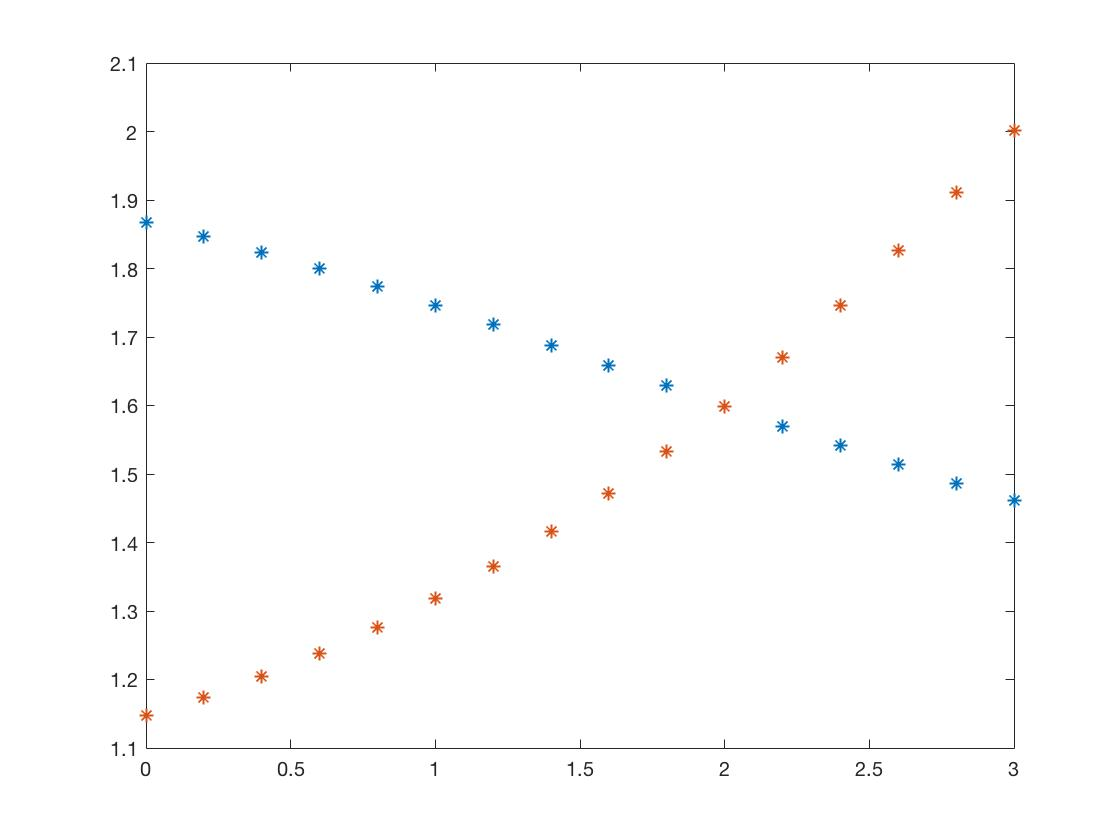
\includegraphics[width=30em, height=20em ]{plot.jpg}



\end{document}